\section{Interfaz}

En esta sección, vamos a mostrar la interfaz de usuario de la aplicación web que se ha desarrollado para servir como \textit{frontend} al sistema de recomendación. Al acceder a la web, el usuario es recibido con un mensaje de bienvenida que le explica sencillamente en qué consiste el sistema.
\\\\
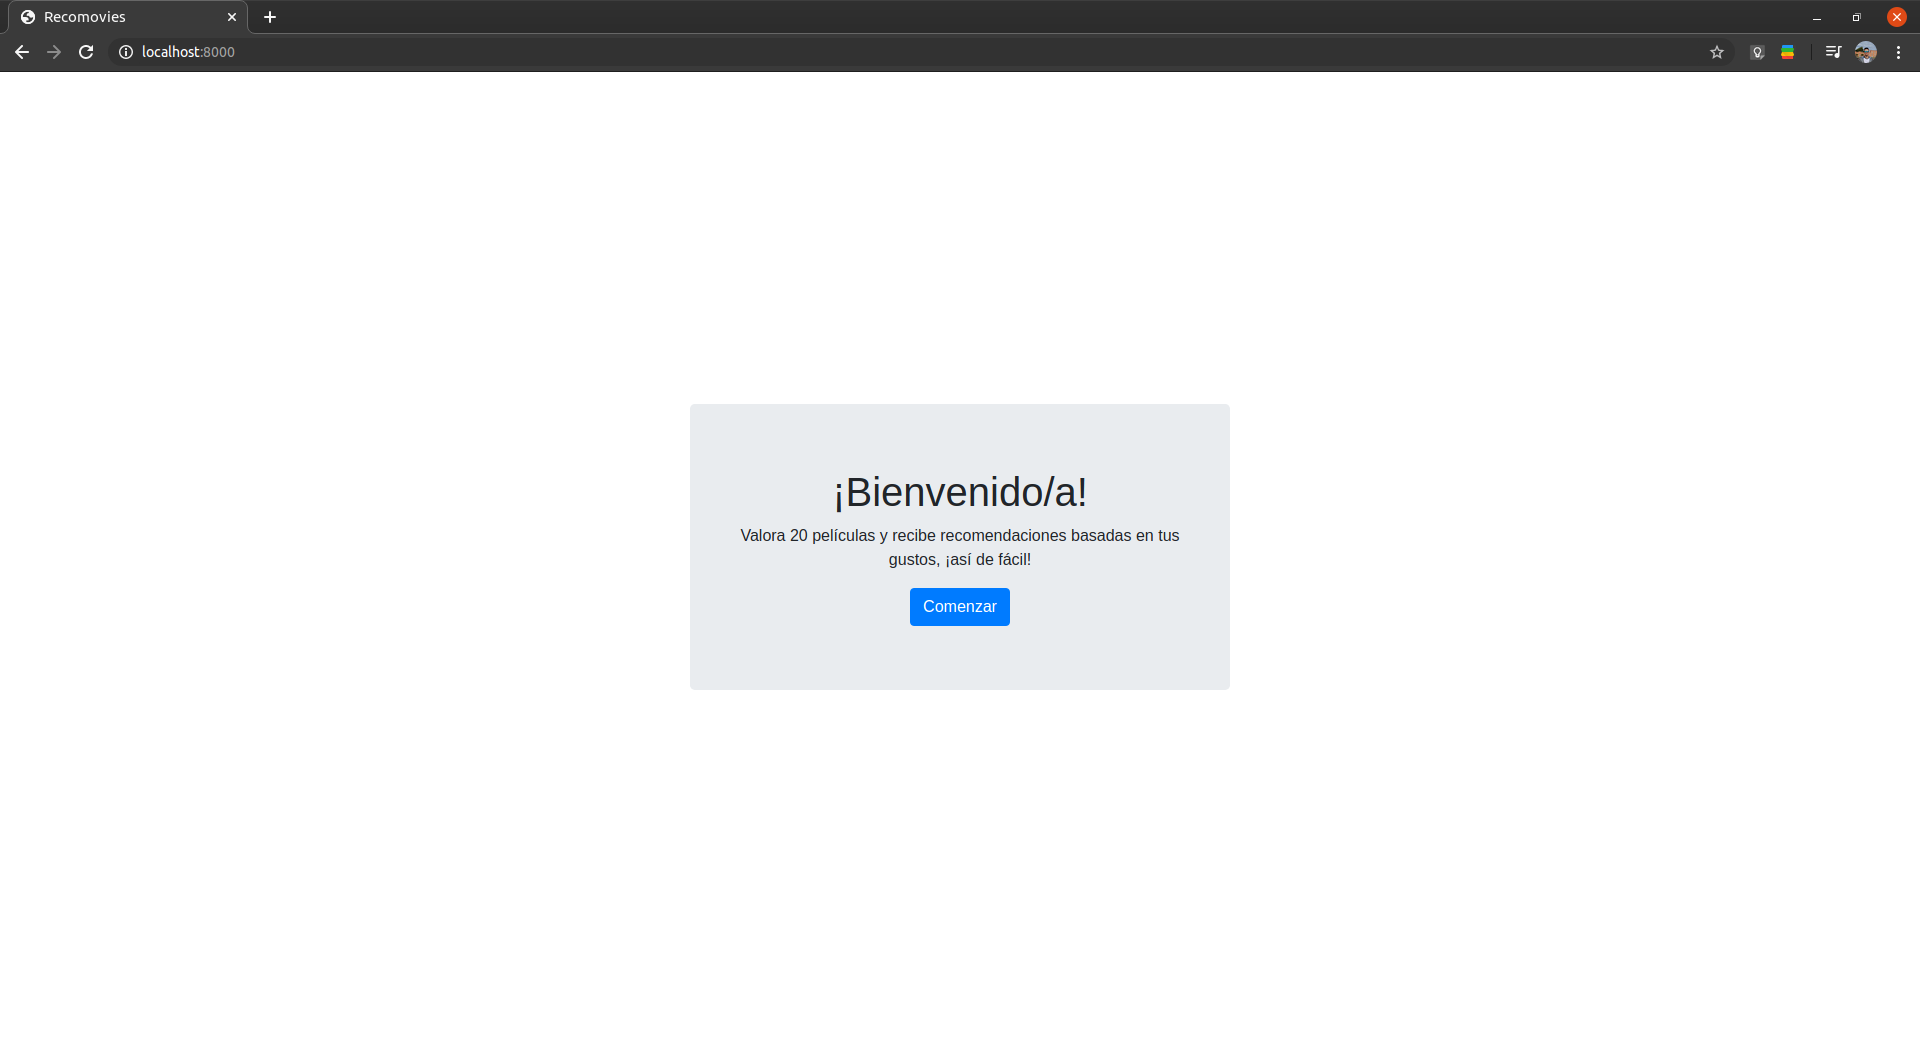
\includegraphics[width=\textwidth,height=\textheight,keepaspectratio]{images/index.png}
\\\\
Cuando el usuario pulsa en el botón de "Comenzar", se crea una nueva sesión para él y se obtienen de forma aleatoria las 20 películas que debe valorar. Estas películas se le muestran de forma secuencial al usuario en pantallas como la que se puede ver a continuación:
\\\\
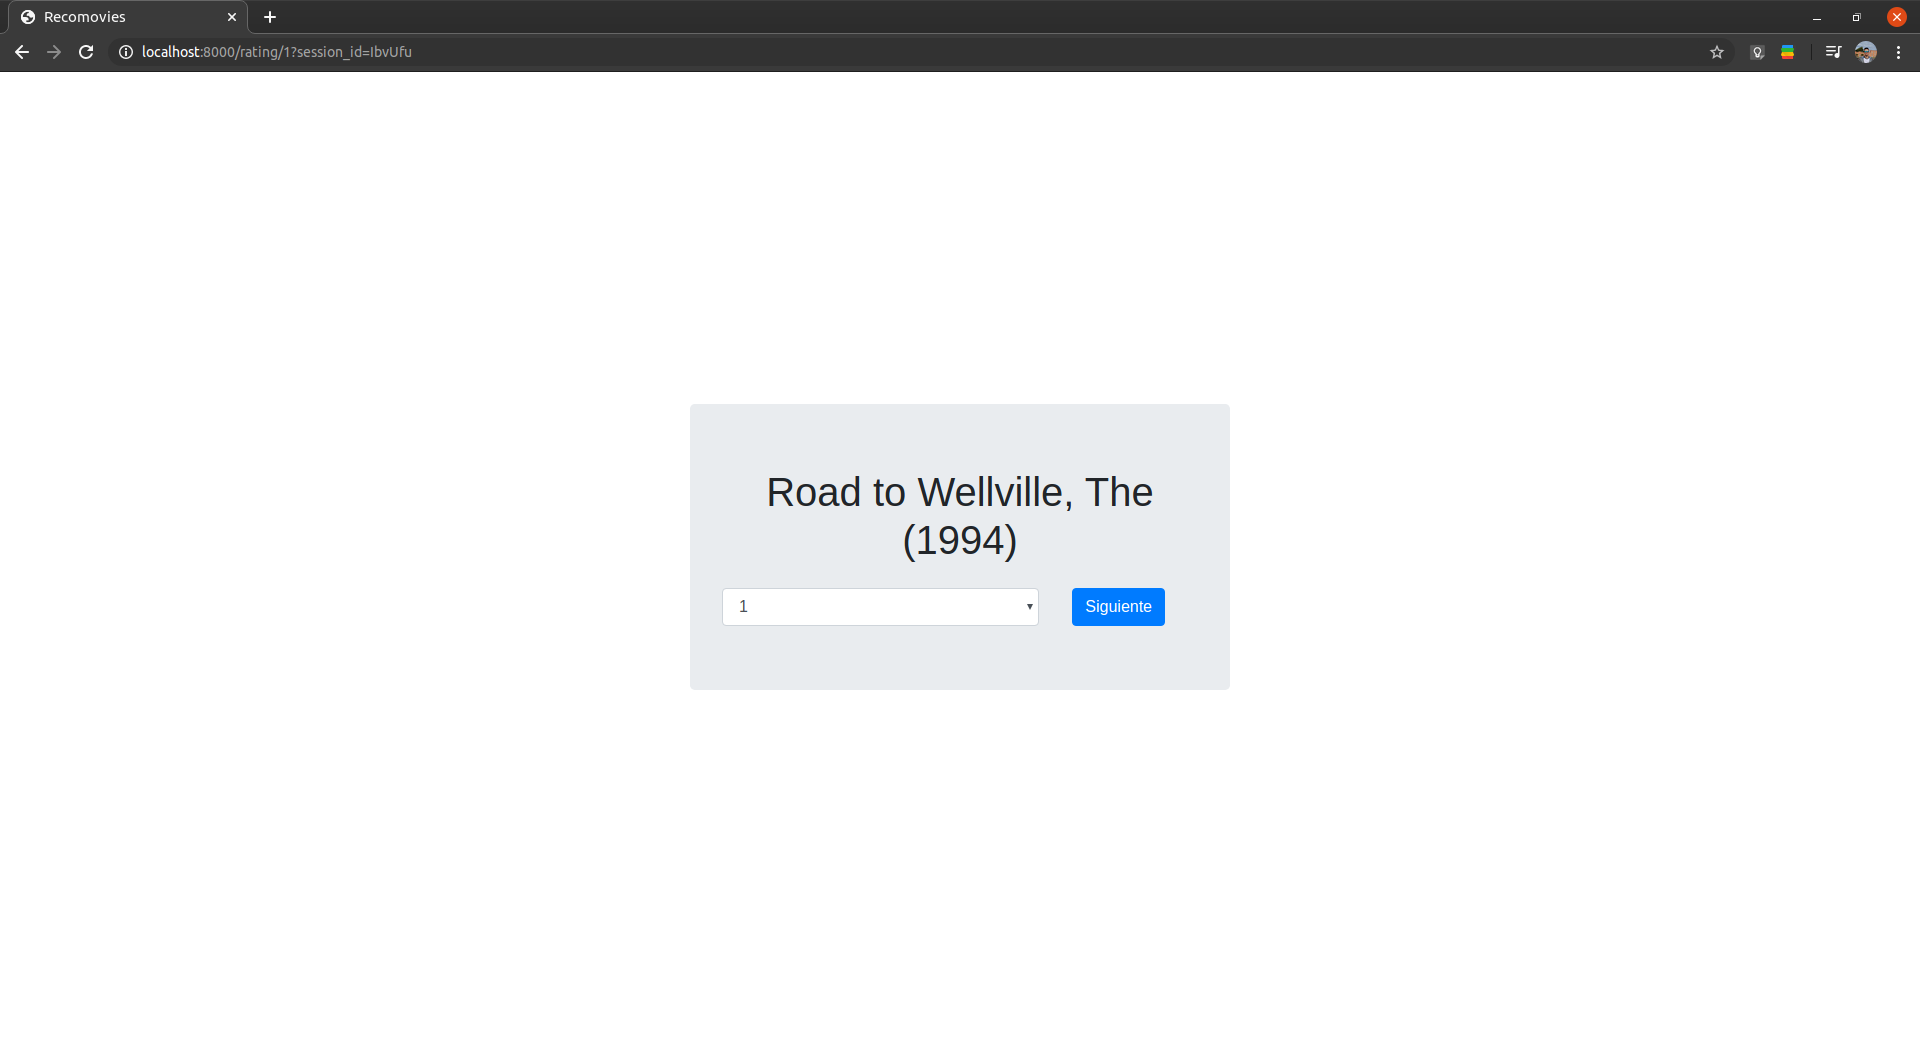
\includegraphics[width=\textwidth,height=\textheight,keepaspectratio]{images/rating.png}
\\\\
Una vez se han valorado las 20 películas, el sistema calcula el vecindario y obtiene las recomendaciones, mostrándoselas al usuario en la pantalla de resultados.
\\\\
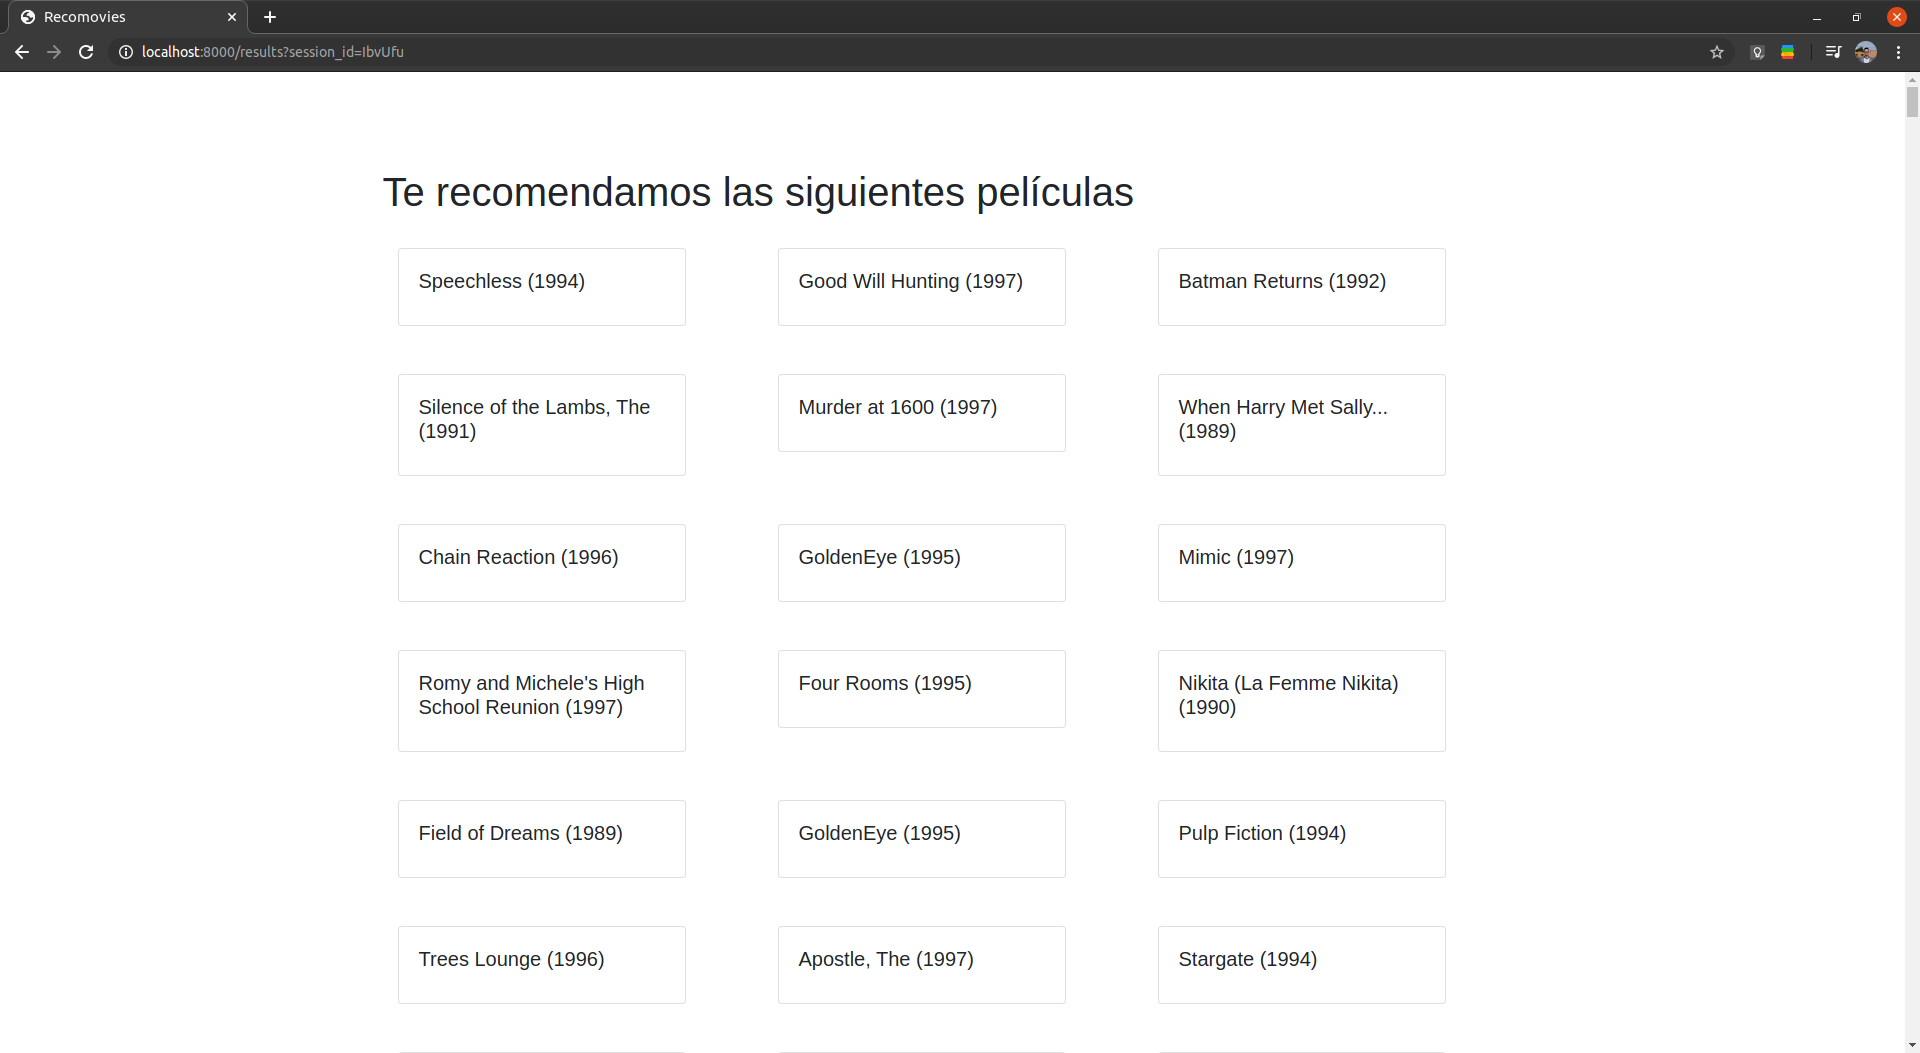
\includegraphics[width=\textwidth,height=\textheight,keepaspectratio]{images/results.png}

\subsection{Manual de uso}

Para ejecutar la aplicación, debe tener una carpeta \textit{data} en la raíz del proyecto que contenga los ficheros \textit{u.data} y \textit{u.item} con los datos. La aplicación leerá estos datos y los cargará en una base de datos SQLite también en la raíz.

Debe tener instaladas en sus sistema las herramientas de Go, con lo que podría lanzar la aplicación con el siguiente comando:

\begin{lstlisting}
go run main.go
\end{lstlisting}

En la terminal se le mostrará el progreso de carga de datos e inicialización del servidor web, tras lo cuál, debería poder acceder a la aplicación con su navegador web a través de la dirección \textit{http://localhost:8000}.